\documentclass[a4paper, oneside, 11pt]{article}

\textwidth 145mm
\topmargin -2mm
\textheight 235mm

\usepackage[czech]{babel}
\usepackage[utf8]{inputenc}
\usepackage[T1]{fontenc}
\usepackage{amsmath}
\usepackage{amsfonts}
\usepackage{amssymb}
\usepackage{graphicx}
\usepackage{fancyhdr}
\usepackage{rotating}
\usepackage{mdwlist}
\usepackage{subfig}
%\usepackage{wasysym}
%\usepackage{siunitx}

\DeclareMathAlphabet{\mathsfb}{T1}{lcmss}{b}{sl}  % tučné bezpatkové písmo

\newcommand{\me}{\mathrm{e}} % Eulerovo cislo
\newcommand{\mi}{\mathrm{i}} % komplexni jednotka
\newcommand{\mj}{\mathrm{j}} % komplexni jednotka
\newcommand{\dif}{\,\mathrm{d}} % diferencial
\newcommand{\mat}[1]{\mathrm{\mathbf{{#1}}}} % tenzor nebo matice
\renewcommand{\vec}[1]{\mbox{\boldmath$#1$}} % vektor
\newcommand{\faz}[1]{{\underline{#1}}} % fazor
\newcommand{\vecfaz}[1]{\mbox{\underline{\boldmath$#1$}}} % fazor vektoru
\newcommand*{\unit}[1]{\ensuremath{\mathrm{\,#1}}} % jednotky
\newcommand{\degree}{\ensuremath{^{\circ}}} % stupne celsia

\renewcommand{\Re}{\mathrm{Re}}
\renewcommand{\Im}{\mathrm{Im}}
\newcommand{\tg}{\mathrm{tg}\ }
\newcommand{\grad}{\mathrm{grad}\ }
\newcommand{\curl}{\mathrm{curl}\ }
\newcommand{\rot}{\mathrm{rot}\ }
\renewcommand{\div}{\mathrm{div}\ }
\newcommand{\const}{\mathrm{const}}
\newcommand{\konst}{\mathrm{konst}}

\newcommand{\fixme}{\begin{center}
\huge{\color{red} \textbf{FIXME: Nutno doplnit!!!}}
\end{center}}

\renewcommand\arraystretch{1.2} % nastaveni vysky bunek tabulek

\makeatletter
\g@addto@macro\@verbatim\footnotesize
\makeatother 

\begin{document}

\renewcommand\thepage{\arabic{page}}
\setcounter{page}{1}
\pagenumbering{arabic}


\noindent {\Huge \textbf{Termoelastická spojka}} \\



\begin{figure}[!hbt]
\centering
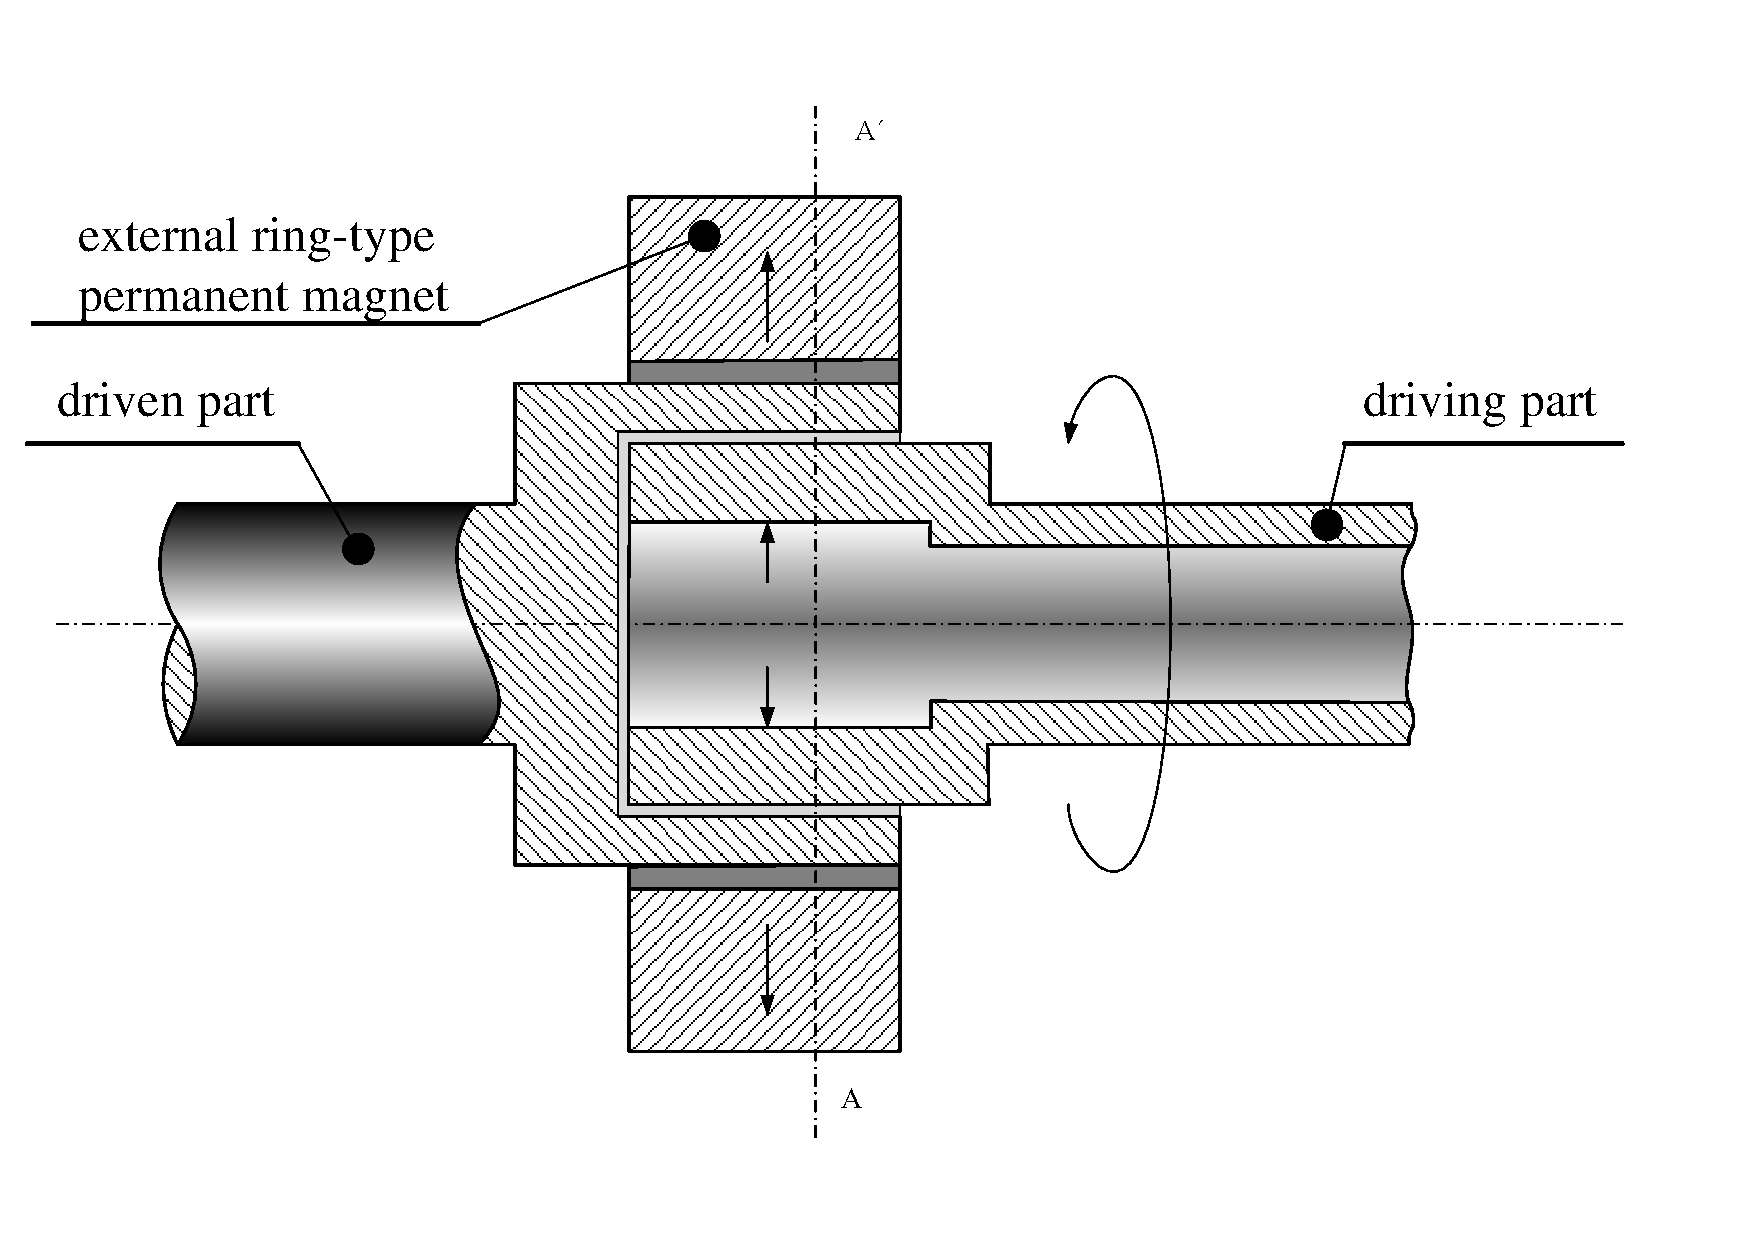
\includegraphics[width=11cm]{spojka.pdf}
\caption{Principiální schéma spojky}
\label{fig:schema_spojky}
\end{figure}

Termoelastická spojka - nástin problematiky - první přiblížení.

\section{Obecný matematický model}
Problém je řešen jako sdružení tří polí. Magnetostatického, teplotního a termoelastického.

Magnetické pole je popsáno rovnicí
$$
\curl (\frac{1}{\mu} (\curl \vec{A} - \vec{B_\mathrm{r}})) - \gamma \vec{v} \times \curl \vec{A} = \vec{0},
$$
kde $\mu$ je permeabilita, $\gamma$ elektrická vodivost, $\vec{v}$ je vektor rychlosti pohybu a $\vec{B_\mathrm{r}}$ je vektor remanence permanentního magnetu.

Teplotní pole je řešeno jako přechodný jev a je popsáno rovnicí
$$
\div (\lambda~\grad T) - \rho c_\mathrm{p} \frac{\partial T}{\partial t} = -p_\mathrm{J},
$$
kde $p_\mathrm{J}$ na pravé straně rovnice jsou Jouleovy ztráty, představující zdroj tepla, $\lambda$ je teplotní vodivost daného materiálu, $\rho$ je hustota a $c_\mathrm{p}$ měrné teplo. V rovnici není uvažován člen $\vec{v} \grad T$.

Termoelasticita je popsána Lamého rovnicí ve tvaru
$$
(\varphi + \psi) \grad(\div \vec{u}) + \psi \Delta \vec{u} - (3\varphi+2\psi) \alpha_{\mathrm{T}} \grad T + \vec{f} = \vec{0} 
$$
kde 
$\varphi=\frac{\nu E}{(1+\nu)(1-2\nu)}$ a $\psi=\frac{E}{2(1+\nu)}$ 

\end{document}
